\documentclass{standalone}
\usepackage{tikz}
\usetikzlibrary{calc}

\begin{document}
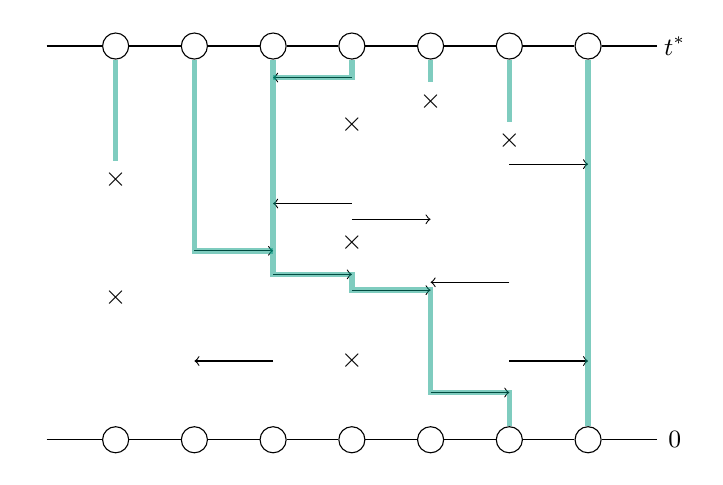
\begin{tikzpicture}

\def \n {7}
\def \height {5}

\newcommand{\obliv}{$\times$}

% Top and bottom nodes
\foreach \s in {1,...,\n} {
  \node (bottom\s) at ( \s , 0) [circle, draw] {};
  \node (top\s) at (\s, \height) [circle, draw] {};
}

% Join nodes together
\foreach \s in {2, ..., \n} {
	\pgfmathparse{\s - 1}
	\draw (bottom\pgfmathresult) -- (bottom\s);
	\draw (top\pgfmathresult) -- (top\s);
}

%Nodes on edges
\node (bottomleft) at (0, 0){};
\node (bottomright) at (\n + 1, 0){};
\node (topleft) at (0, \height){};
\node (topright) at (\n + 1, \height){};
\draw (bottomleft) -- (bottom1);
\draw (bottomright) -- (bottom\n);
\draw (topleft) -- (top1);
\draw (topright) -- (top\n);


% Oblivious Updates

\node (v1o1) at (1, 3.3) {\obliv};
\node (v1o2) at (1, 1.8) {\obliv};

\node (v4o1) at (4, 4) {\obliv};
\node (v4o2) at (4, 2.5) {\obliv};
\node (v4o3) at (4, 1) {\obliv};

\node (v5o1) at (5, 4.3) {\obliv};

\node (v6o1) at (6, 3.8) {\obliv};

% Directional Updates

\draw [->] (2, 2.4) -- (3, 2.4);

\draw [->] (3, 2.1) -- (4, 2.1);
\draw [->] (3, 1) -- (2, 1);

\draw [->] (4, 4.6) -- (3, 4.6);
\draw [->] (4, 3) -- (3, 3);
\draw [->] (4, 2.8) -- (5, 2.8);
\draw [->] (4, 1.9) -- (5, 1.9);

\draw [->] (5, 0.6) -- (6, 0.6);

\draw [->] (6, 3.5) -- (7, 3.5);
\draw [->] (6, 2) -- (5, 2);
\draw [->] (6, 1) -- (7, 1);

% Upper vertex labels
% \node at (4, \height + 0.5) [] {$i$};

% Time labels
\node at (8.1,0) [] {\small$0$};
\node at (8.1,\height) [] {\small$t^*$};

% Percolation
\definecolor{history}{rgb}{0, 0.6, 0.5}
\tikzstyle{every path}=[draw, line width = 2pt, opacity = 0.5, history]
\draw (top1) -- (v1o1);
\draw (top2) -- (2, 2.4) -- (3, 2.4);

\draw (top3) -- (3, 2.1)--(4, 2.1) -- (4, 1.9) -- (5, 1.9) -- (5, 0.6) -- (6, 0.6) -- (bottom6);

\draw (top4) -- (4, 4.6) -- (3, 4.6);

\draw (top5) -- (v5o1);

\draw (top6) -- (v6o1);

\draw (top7) -- (bottom7);

\end{tikzpicture}
\end{document}